\chapter{Selecting the Best Sigma Parameter}
\label{ch:sigma_selection}

\section{Overview}

The upsampling factor $\sigma$ is among the most impactful parameters in FINUFFT. It determines the size of the internal FFT grid relative to the output grid, and thus directly controls the memory footprint, cache behaviour, and compute cost of the transform. This chapter investigates how to select $\sigma$ optimally for a given input configuration and accuracy requirement.

\section{The Role of $\sigma$ in FINUFFT}

The upsampling factor $\sigma$ controls the size of the internal uniform FFT grid, which has $\sigma N$ points per dimension relative to the $N$ requested output modes. Increasing $\sigma$ enlarges the FFT grid, raising FFT cost, but simultaneously relaxes the accuracy requirement on the spreading kernel, permitting a smaller kernel half-width $w$. Because $w$ decreases and the grid size increases as $\sigma$ grows, there exists a value of $\sigma$ that minimises total transform cost for a given problem size, dimension, and tolerance.

\section{Current Heuristic for $\sigma$ Selection}
The current FINUFFT heuristic for $\sigma$ selection is a simple lookup: it returns one of only two possible values, $\sigma \in \{1.25, 2.00\}$. By default it returns $1.25$, but switches to $2.00$ when the point density $\rho = M/N$ exceeds a fixed threshold, or when the requested tolerance $\varepsilon$ is too tight for $\sigma = 1.25$ to reach. All upsampling factors in between are never considered, even though the true optimal $\sigma$ for a given problem often lies in the interior of $[1.25, 2.00]$.

\section{Cost Model}
This section describes cost models for FFT and spreading steps of the algorithm.

\subsection{Estimating Spreading Cost}

The spreading step accumulates contributions from each of the $M$ non-uniform source points onto a $w^d$ neighbourhood of grid cells. The minimum kernel half-width $w$ required to achieve tolerance $\varepsilon$ at upsampling $\sigma$ in $d$ dimensions is
\begin{equation}
    w = \left\lceil \frac{\log\!\left(\dfrac{0.18 \cdot 1.4^{d-1}}{\varepsilon}\right)}{\pi \sqrt{1 - 1/\sigma}} + 1 \right\rceil.
    \label{eq:kernel_width}
\end{equation}
The theoretical spreading cost is therefore proportional to $M w^d$. In practice the inner loop is vectorised, so the per-point work scales as $\lceil w / W_{\mathrm{simd}} \rceil \cdot w^{d-1}$, where $W_{\mathrm{simd}}$ is the SIMD vector width in grid points.

\subsection{Estimating FFT Cost}

The FFT operates on the upsampled grid of total size $\tilde{N} = \mathrm{next235}(\sigma N)^d$, where $\mathrm{next235}(x)$ denotes the smallest integer $\geq x$ whose only prime factors are $2$, $3$, and $5$. Rounding up to such a highly composite number ensures the FFT can be decomposed into small radix-2, -3, and -5 butterflies, which most FFT libraries handle efficiently. The grid contributes $\mathcal{O}(\tilde{N} \log \tilde{N})$ operations, though the precise constant depends on the chosen FFT backend and cache effects, so this estimate is best treated as an asymptotic guide.


\begin{figure}[h]
    \centering
    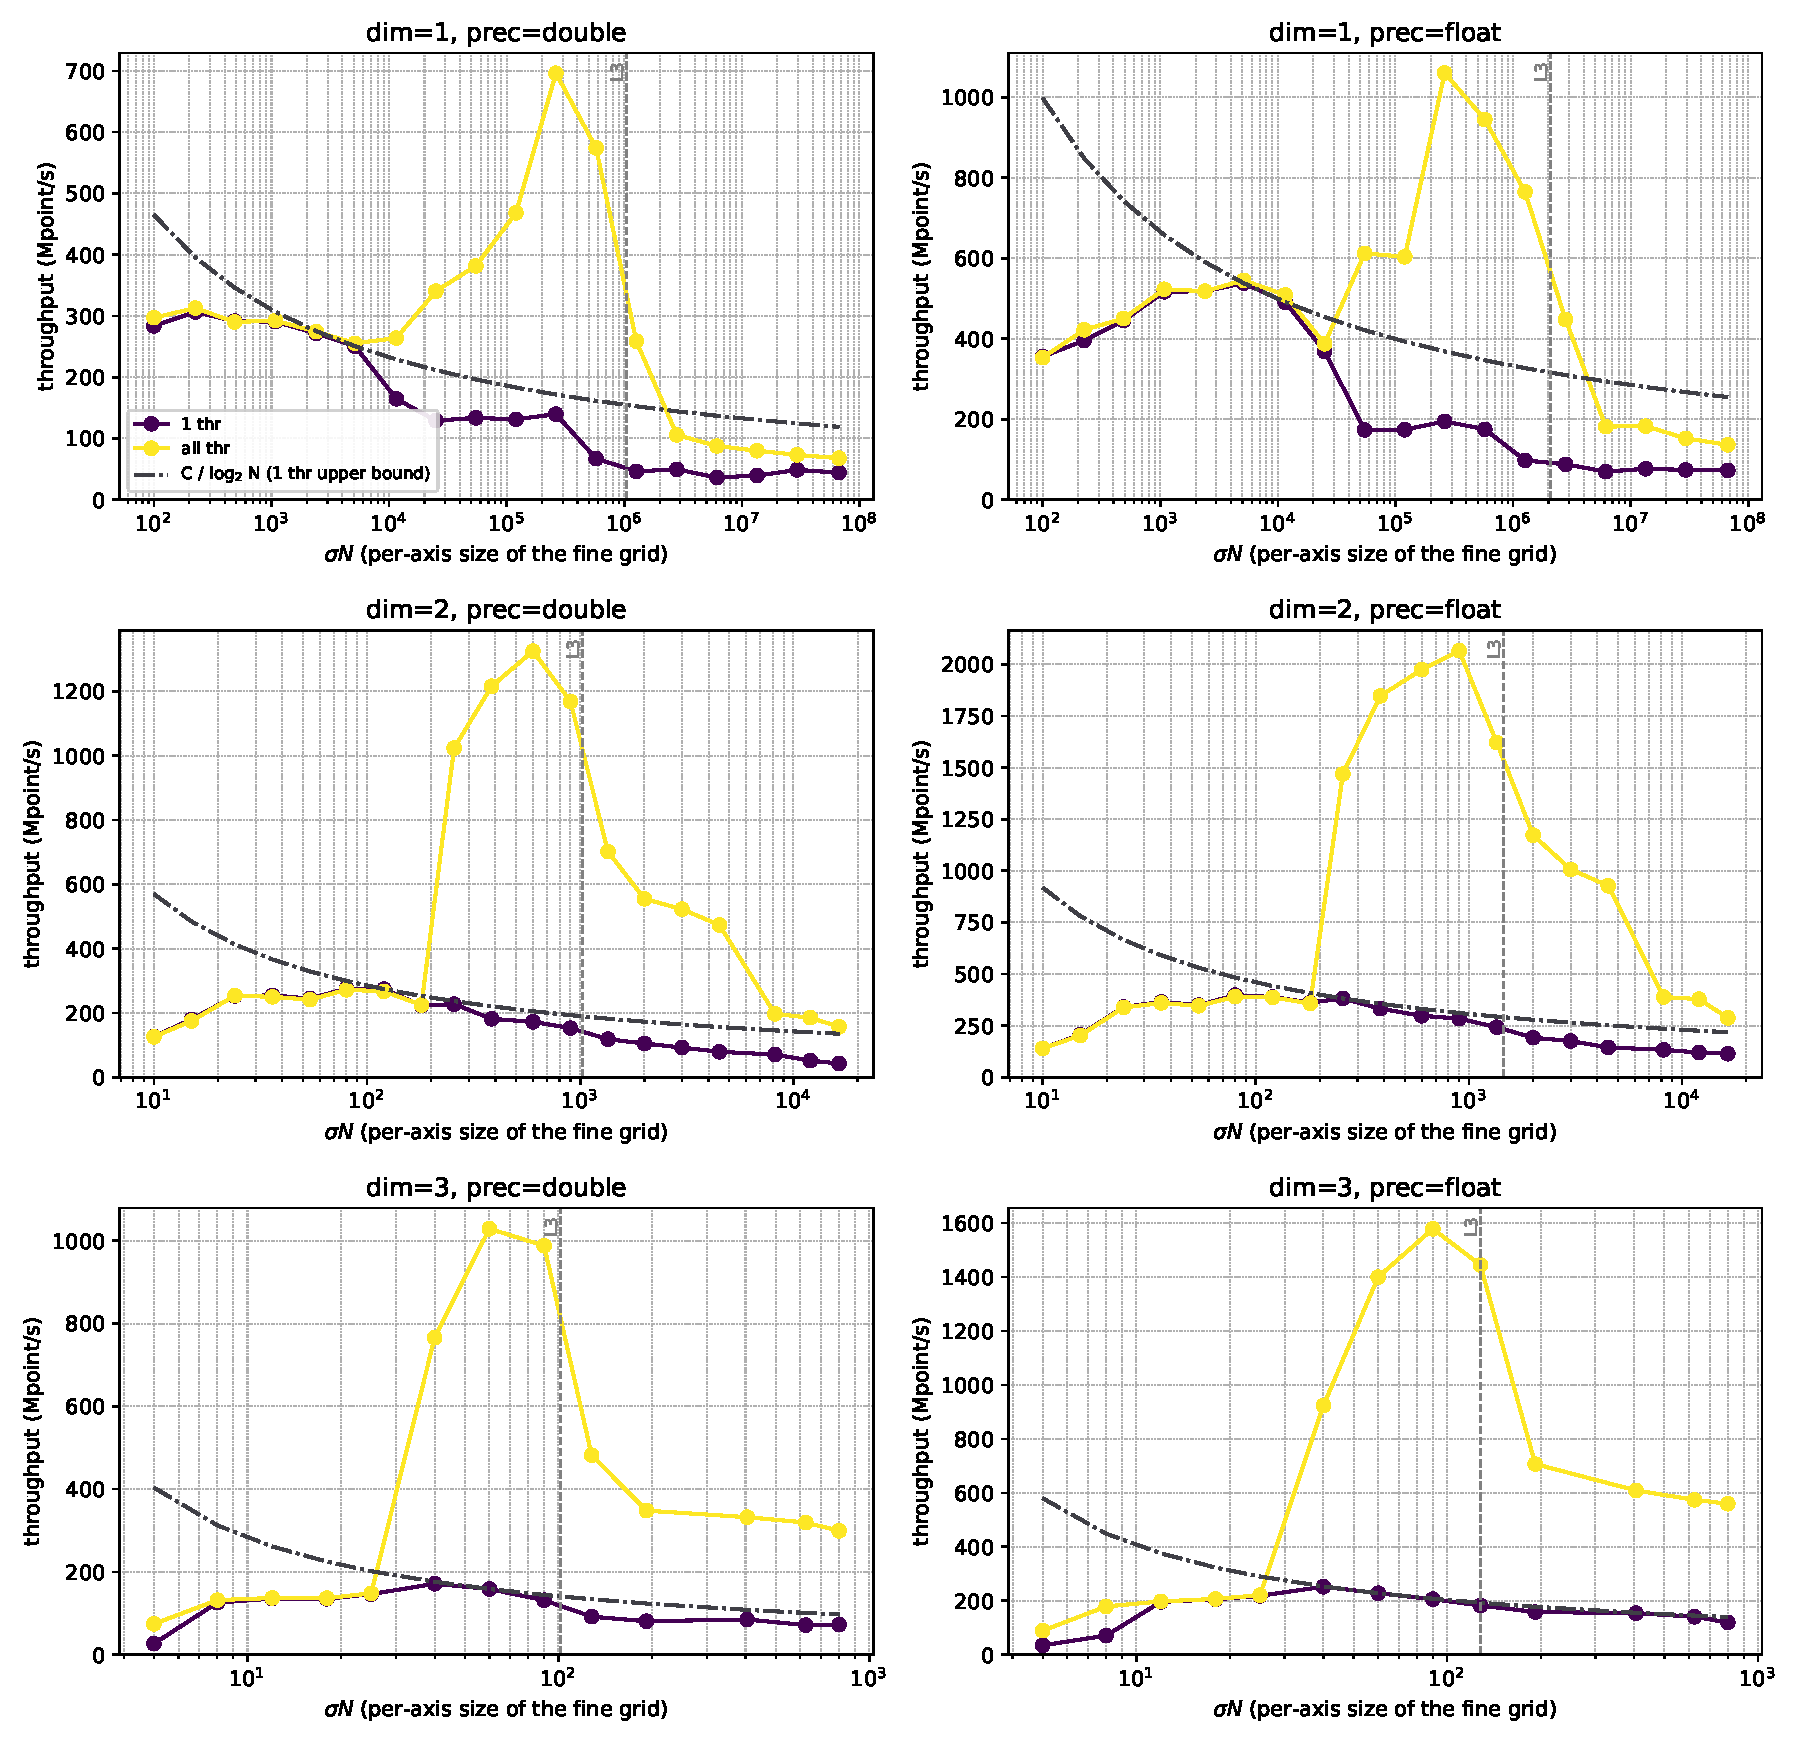
\includegraphics[width=\textwidth]{figures/fft_cost/ducc_fft_scaling.pdf}
    \caption{DUCC FFT throughput for complex-to-complex transforms in one, two
    and three dimensions at single and double precision on 1 and 16 threads.
    }
    \label{fig:ducc_fft_scaling}
\end{figure}

\section{Analytical Measurements}
All timing measurements in this chapter were collected using Google Benchmark~\cite{googlebenchmark}. Google Benchmark provides statistical rigor by running each fixture repeatedly and reporting mean and standard deviation, automatically discarding warm-up iterations and compensating for clock resolution. It also integrates with hardware performance counters, enabling cycle-accurate comparisons across configurations. These properties make it well-suited for the fine-grained measurements of spreading and FFT cost required here. All runs were performed on a single machine: an Intel Xeon E5-2698 v4 CPU (2.20\,GHz, 20 cores / 40 threads, single socket, 50\,MiB L3 cache).

\subsection{Validating FFT Cost Model}

Figure~\ref{fig:ducc_fft_scaling} tests the $\mathcal{O}(\tilde{N} \log \tilde{N})$ asymptotic guide
against measured DUCC FFT throughput. If the cost per butterfly were constant, the achieved
throughput would decay as $1/\log_2 \tilde{N}$, drawn as the dash-dotted reference in
each panel. The measurements depart from the model in two regimes.
First, for small transforms the throughput increases with grid size, because the fixed
per-call overhead is amortised over an increasing number of points. For larger transforms
the single-threaded throughput follows the $1/\log_2 \tilde{N}$ trend. The throughput of a
transform that uses all threads on the machine, however, keeps increasing as long as the
whole transform fits in the L3 cache.
DUCC implements the FFT with a mixed-radix Cooley--Tukey algorithm, which performs only
$\mathcal{O}(\log \tilde{N})$ pralelized over multiple threads arithmetic operations, per element and is therefore limited by
memory bandwidth rather than by arithmetic throughput. As long as all points fit in the L3
cache, the successive passes over the array are served without loads from main memory. Once
the array spills into main memory, the parallel version also settles onto the
$1/\log_2 \tilde{N}$ trend.

\subsection{Validating the Spreading Cost Model}

To validate the $w^d$ scaling predicted by the model, spreading time was measured across one and two dimensions for a range of $\sigma$ values at tolerance $\varepsilon = 10^{-6}$. As shown in Figures~\ref{fig:spreading_1d} and~\ref{fig:spreading_2d}, the theoretical curves follow the same trajectory as the measurements, including the location of the minimum. This confirms that the model can be used to identify the value of $\sigma$ that minimises spreading cost without exhaustive profiling.

\begin{figure}[h]
    \centering
    \begin{subfigure}[b]{0.48\textwidth}
        \centering
        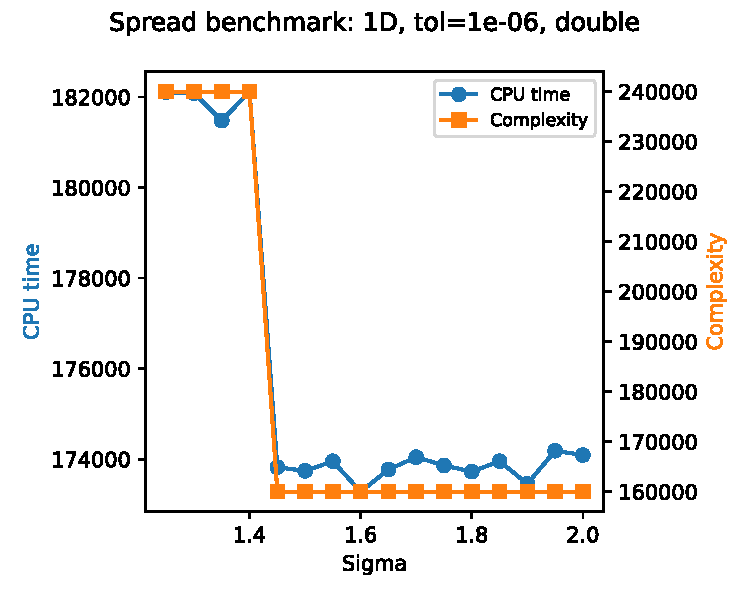
\includegraphics[width=\textwidth]{figures/spreading/1d1e-6d.pdf}
        \caption{1D}
        \label{fig:spreading_1d}
    \end{subfigure}
    \hfill
    \begin{subfigure}[b]{0.48\textwidth}
        \centering
        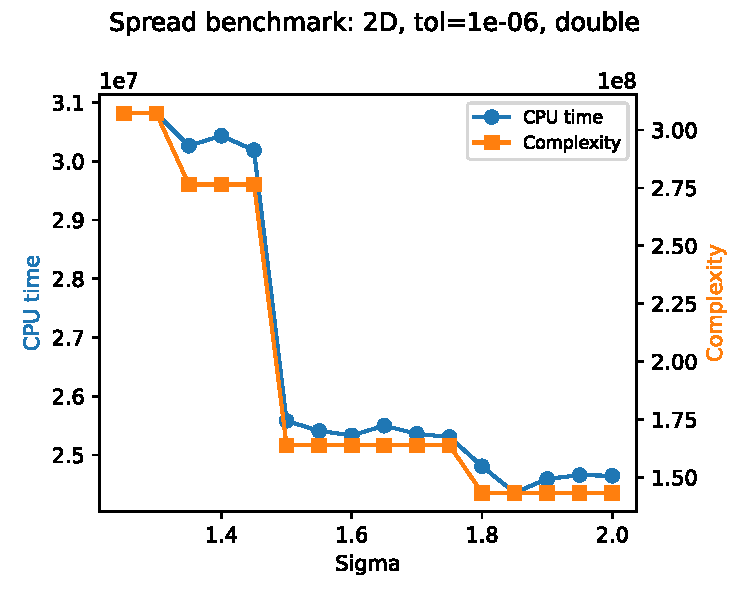
\includegraphics[width=\textwidth]{figures/spreading/2d1e-06d.pdf}
        \caption{2D}
        \label{fig:spreading_2d}
    \end{subfigure}
    \caption{Spreading cost versus $\sigma$ at $\varepsilon = 10^{-6}$. The solid line is the prediction from \eqref{eq:kernel_width}; points are measured timings.}
    \label{fig:spreading_validation}
\end{figure}

